\documentclass[tikz,border=8pt]{standalone}
% Shared look for every TikZ diagram. Load with % Shared look for every TikZ diagram. Load with % Shared look for every TikZ diagram. Load with \input{../../tools/tikz-style.tex}
\usepackage[T1]{fontenc}
\usepackage{lmodern}
\renewcommand{\sfdefault}{lmr}  % diagrams use the same serif as the text
\usetikzlibrary{arrows.meta, positioning, shapes.geometric, calc, fit, backgrounds}
\definecolor{cblue}{HTML}{4C78A8}
\definecolor{corange}{HTML}{F58518}
\definecolor{cgreen}{HTML}{54A24B}
\definecolor{cred}{HTML}{E45756}
\definecolor{cpurple}{HTML}{B279A2}
\definecolor{cgrey}{HTML}{6B6B6B}
\tikzset{
  every picture/.style={font=\sffamily, line width=1.2pt},
  box/.style={draw=#1, fill=#1!12, rounded corners=4pt, align=center, inner sep=7pt, minimum height=1.1cm},
  box/.default=cgrey,
  arrow/.style={-{Stealth[length=3mm]}, draw=cgrey, line width=1.4pt},
  title/.style={font=\sffamily\bfseries\Large},
  note/.style={font=\sffamily\small, text=cgrey, align=center},
}
\AtBeginDocument{\hyphenpenalty=10000 \exhyphenpenalty=10000}

\usepackage[T1]{fontenc}
\usepackage{lmodern}
\renewcommand{\sfdefault}{lmr}  % diagrams use the same serif as the text
\usetikzlibrary{arrows.meta, positioning, shapes.geometric, calc, fit, backgrounds}
\definecolor{cblue}{HTML}{4C78A8}
\definecolor{corange}{HTML}{F58518}
\definecolor{cgreen}{HTML}{54A24B}
\definecolor{cred}{HTML}{E45756}
\definecolor{cpurple}{HTML}{B279A2}
\definecolor{cgrey}{HTML}{6B6B6B}
\tikzset{
  every picture/.style={font=\sffamily, line width=1.2pt},
  box/.style={draw=#1, fill=#1!12, rounded corners=4pt, align=center, inner sep=7pt, minimum height=1.1cm},
  box/.default=cgrey,
  arrow/.style={-{Stealth[length=3mm]}, draw=cgrey, line width=1.4pt},
  title/.style={font=\sffamily\bfseries\Large},
  note/.style={font=\sffamily\small, text=cgrey, align=center},
}
\AtBeginDocument{\hyphenpenalty=10000 \exhyphenpenalty=10000}

\usepackage[T1]{fontenc}
\usepackage{lmodern}
\renewcommand{\sfdefault}{lmr}  % diagrams use the same serif as the text
\usetikzlibrary{arrows.meta, positioning, shapes.geometric, calc, fit, backgrounds}
\definecolor{cblue}{HTML}{4C78A8}
\definecolor{corange}{HTML}{F58518}
\definecolor{cgreen}{HTML}{54A24B}
\definecolor{cred}{HTML}{E45756}
\definecolor{cpurple}{HTML}{B279A2}
\definecolor{cgrey}{HTML}{6B6B6B}
\tikzset{
  every picture/.style={font=\sffamily, line width=1.2pt},
  box/.style={draw=#1, fill=#1!12, rounded corners=4pt, align=center, inner sep=7pt, minimum height=1.1cm},
  box/.default=cgrey,
  arrow/.style={-{Stealth[length=3mm]}, draw=cgrey, line width=1.4pt},
  title/.style={font=\sffamily\bfseries\Large},
  note/.style={font=\sffamily\small, text=cgrey, align=center},
}
\AtBeginDocument{\hyphenpenalty=10000 \exhyphenpenalty=10000}

\begin{document}
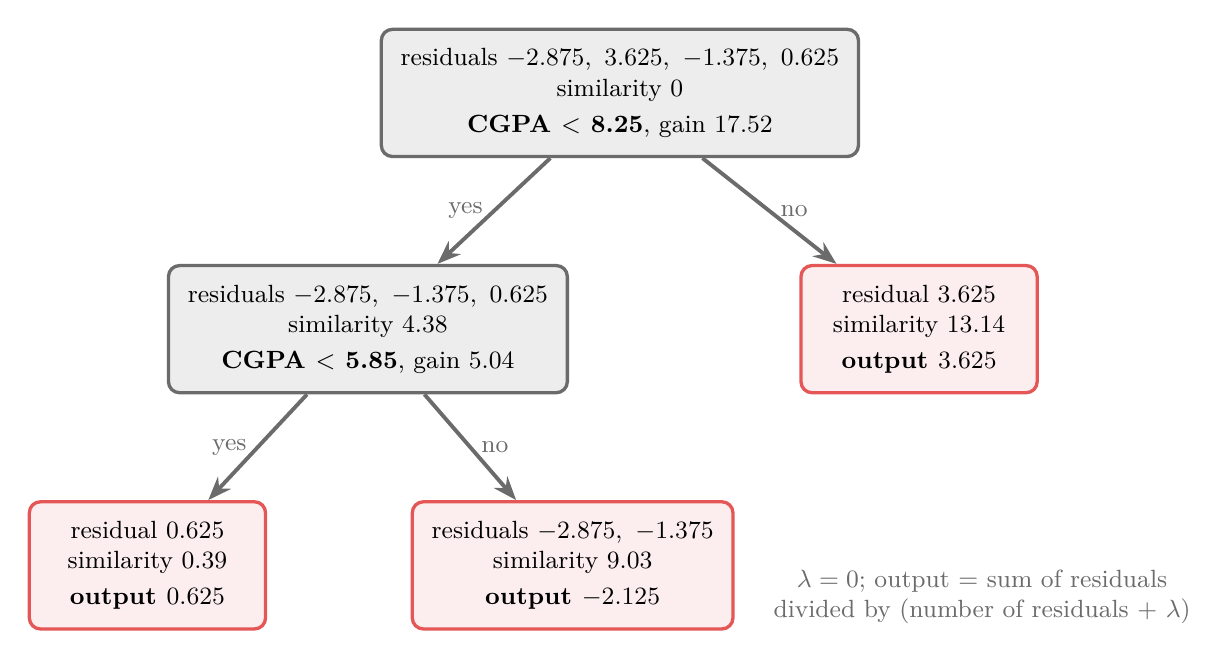
\begin{tikzpicture}[n/.style={box=cgrey, align=center, font=\sffamily\small, minimum width=3.6cm},
  l/.style={box=cblue, align=center, font=\sffamily\small, minimum width=3.0cm}]
  \node[n] (r) at (0,0) {residuals $-2.875,\ 3.625,\ -1.375,\ 0.625$\\similarity $0$\\[2pt] \textbf{CGPA $<$ 8.25}, gain $17.52$};
  \node[n] (a) at (-3.2,-3) {residuals $-2.875,\ -1.375,\ 0.625$\\similarity $4.38$\\[2pt] \textbf{CGPA $<$ 5.85}, gain $5.04$};
  \node[l, draw=cred, fill=cred!10] (b) at (3.8,-3) {residual $3.625$\\similarity $13.14$\\[2pt] \textbf{output $3.625$}};
  \node[l, draw=cred, fill=cred!10] (c) at (-6.0,-6) {residual $0.625$\\similarity $0.39$\\[2pt] \textbf{output $0.625$}};
  \node[l, draw=cred, fill=cred!10] (d) at (-0.6,-6) {residuals $-2.875,\ -1.375$\\similarity $9.03$\\[2pt] \textbf{output $-2.125$}};
  \draw[arrow] (r) -- node[note, left] {yes} (a); \draw[arrow] (r) -- node[note, right] {no} (b);
  \draw[arrow] (a) -- node[note, left] {yes} (c); \draw[arrow] (a) -- node[note, right] {no} (d);
  \node[note] at (4.6,-6.4) {$\lambda = 0$; output = sum of residuals\\divided by (number of residuals $+\ \lambda$)};
\end{tikzpicture}
\end{document}
